% vim: set tw=78 tabstop=4 shiftwidth=4 aw ai:

\chapter{Protocol Measurement and Analysis in Peer-to-Peer Systems}
\label{chapter:proto-measure}

Based on BitTorrent's success story (it has managed to become the number one
protocol of the internet in a matter of years), the scientific community has
delved heavily in analysing, understanding and improving its performance.
Research focus has ranged from measurements~\cite{measurement-study} to
protocol improvements~\cite{bt-impr}, from social
networking~\cite{tribler-social} to moderation
techniques~\cite{measurements-analysis}, from content distribution
enhancements~\cite{bitos} to network infrastructure impact~\cite{bt-impact}.

We undertook a novel approach involving client-side information collection
regarding client and protocol implementation. We have instrumented a
libtorrent-rasterbar
client\footnote{http://www.rasterbar.com/products/libtorrent/} and a
Tribler\footnote{http://www.tribler.org/trac/} client to provide verbose
information regarding BitTorrent protocol implementation. These results are
collected and subsequently processed and analysed through a rendering
interface.

Our aim is to measure and analyze protocol messages while in real-world
environments. As described in Chapter~\ref{chapter:virt-infra}, a virtualized
infrastructure had been used for realistic environments; apart from that
clients and trackers running in a real-world swarm have been used and
instrumented to provide valuable protocol information and parameters. No
simulators have been used for collecting, measuring and analyzing protocol
parameters, rather a ``keep it real as much as possible'' approach.
Information, messages and parameters are collected directly from peers and
tracker that are part of a real-world Peer-to-Peer swarm.

The action chronology for measuring parameters had been collecting data,
parsing and storing it and then subjecting protocol parameters to processing
and analysis. The rest of this chapter presents the measured parameters,
approaches to collecting, parsing and storing information into an ``easy to be
used'' format and then putting it to analysis and interpretation.

\section{BitTorrent Messages and Parameters}
\label{sec:proto-measure:protocol-messages}

Analysis of BitTorrent client-centric behavior and, to some extent, swarm
behavior, is based on BitTorrent protocol
messages\footnote{http://www.bittorrent.org/beps/bep\_0003.html}. Messages are
used for handshaking, closing the connection, requesting and receiving data.

The BitTorrent client will generate at startup a unique identifier of itself,
known as \textit{peer id}. This is client dependent, each client encoding a
peer id based on its own implementation.

\subsection{Protocol Messages}

Each torrent is exclusively identified by a 20-byte SHA1 hash of the value of
the info key from the torrent file dictionary which is defined as \textit{info
hash}. The peer id and info hash values are important in the TCP connection
establishing and are typically logged by trackers.

The handshake is the first sent message. It uses the format:
\begin{verbatim}
<length><protocol><reserved><info_hash><peer_id>
\end{verbatim}

The protocol parameter represents the protocol identifier string and the
length parameter represents the protocol name length. Reserved represents
eight reserved bytes whose bits can be used to modify the behavior of the
protocol. Standard implementations use this as zero-filled.
\texttt{info\_hash} represents the identifier of the shared resource that is
desired by the initiator of the connection. \texttt{peer\_id} represents the
initiator's unique identifier.

The receiver of the handshake must verify the \texttt{info\_hash} in order to
decide if it can serve it. If it is not currently serving, it will drop the
connection.  Otherwise, the receiver will send its own handshake message to
the initiator of the connection. If the initiator receives a handshake whose
\texttt{peer\_id} does not match with the expected one -- it must keep a list
with peers addresses and ports and their corresponding \texttt{peer\_id}'s --
then it also must drop the connection.

Remaining protocol messages have the format:
\begin{verbatim}
<length><message ID><payload>
\end{verbatim}

The length prefix is a four byte big-endian value representing the sum of message ID and payload sizes. The message ID is a single decimal byte. The payload is message dependent.

\begin{itemize}

  \item \textbf{keep-alive} (\texttt{$<$len=0000$>$}) \\
    The Keep-alive message is the only message without any message ID and
    payload.  It is sent to maintain the connection alive if no other message
    has been sent for a given amount of time. The amount of time is about two
    minutes.

  \item \textbf{choke} (\texttt{$<$len=0001$>$$<$id=0$>$}) \\
    The Choke message is sent when the client wants to choke a remote peer.

  \item \textbf{unchoke} (\texttt{$<$len=0001$>$$<$id=1$>$}) \\
    The Unchoke message is sent when the client wants to unchoke a remote peer.

  \item \textbf{interested} (\texttt{$<$len=0001$>$$<$id=2$>$}) \\
    The Interested message is sent when the client is interested in something
    that the remote peer has to offer.

  \item \textbf{not interested} (\texttt{$<$len=0001$>$$<$id=2$>$}) \\
    The Not interested message is sent when the client is not interested in
    anything that the remote peer has to offer.

  \item \textbf{have} (\texttt{$<$len=0005$>$$<$id=4$>$$<$piece index$>$}) \\
    The piece index is a 4 bytes value representing the zero-based index of a
    piece that has just been successfully downloaded and verified via its hash
    value present in the torrent file.

  \item \textbf{bitfield} (\texttt{$<$len=0001+X$>$$<$id=5$>$$<$bitfield$>$}) \\
    The bitfield message may only be sent immediately after the handshake
    sequence has occurred and before any other message is sent. It is optional
    and need not be sent if a client has no pieces. The Bitfield payload has
    the length X and its bits represent the pieces that have been successfully
    downloaded. The high bit in the first byte corresponds to piece index 0. A
    set bit indicates a valid and available piece, and a cleared bit indicates
    a missing piece. Any spare bits are set to zero.

  \item \textbf{request}
  (\texttt{$<$len=0013$>$$<$id=6$>$$<$index$>$$<$begin$>$$<$length$>$}) \\
    The Request message is sent when requesting a block. Index is the
    zero-based index of the piece containing the requested block, begin is the
    block offset inside the piece and length represents the block size.

  \item \textbf{piece}
  (\texttt{$<$len=0009+X$>$$<$id=7$>$$<$index$>$$<$begin$>$$<$block$>$}) \\
    The Piece message is sent when delivering a block to an interested peer.
    Index is the zero-based index of the piece containing the delivered block,
    begin is the block offset inside the piece and block represents the
    X-sized block data.

  \item \textbf{cancel}
  (\texttt{$<$len=0013$>$$<$id=8$>$$<$index$>$$<$begin$>$$<$length$>$}) \\
    The Cancel message is sent when canceling a block request sent before.
    Index is the zero-based index of the piece containing the requested block,
    begin is the block offset inside the piece and length represents the block
    size.

  \item \textbf{port} (\texttt{$<$len=0003$>$$<$id=9$>$$<$listen port$>$}) \\
The Port message is sent by clients that implement a DHT tracker. The listen port is the port of the client's DHT node listening on.

\end{itemize}

Swarm measured data are usually collected from trackers. While this offers a
global view of the swarm it has little information about client-centric
properties such as protocol implementation, neighbour set, number of connected
peers, etc. A more thorough approach has been presented by Iosup et
al.~\cite{corr-overlay}, using network probes to interrogate various clients.

Our approach, while not as scalable as the above mentioned one, aims to collect
client-centric data, store and analyse it in order to provide information on
the impact of network topology, protocol implementation and peer
characteristics. Our infrastructure provides micro-analysis, rather than
macro-analysis of a given swarm. We focus on detailed peer-centric properties,
rather than less-detailed global, tracker-centric information. The data
provided by controlled instrumented peers in a given swarm is retrieved,
parsed and stored for subsequent analysis.

We differentiate between two kinds of BitTorrent messages \textit{status
messages}, which clients provide periodically to report the current session’s
download state, and \textit{verbose messages} that contain protocol messages
exchanged between peers (chokes, unchokes, peer connections, pieces transfer
etc.).

Another type of messages are those provided by tracker logging. Tracker-based
messages provide an overall view of the entire swarm, albeit at the cost of
less-detailed information. Tracker logging typically consists of periodic
messages sent by clients as announce messages. However, these messages' period
is quite large (usually 30 minutes -- 1800 seconds) resulting in less detailed
information. Their overall swarm vision is an important addition to status and
verbose client messages.

\subsection{Measured Data and Parameters}

Data and parameters measured are those particular to BitTorrent clients and
swarms, that provide support for evaluation and improvements at protocol level.
The measured parameters are described in the
Table~\ref{tab:proto-measure:status-messages-params},
Table~\ref{tab:proto-measure:verbose-messages-params} and
Table~\ref{tab:proto-measure:tracker-messages-params}, depending
on their source (either status messages, verbose messages or tracker
messages).

\begin{table}[htb]
  \centering
  \caption{Parameters from Status Messages}
  \label{tab:proto-measure:status-messages-params}
  \begin{tabular}{@{}ll@{}}
    \toprule
      \textbf{Parameter} & \textbf{Explanation} \\
    \midrule
      Download speed & Current peer download speed -- number of bytes
      received \\
      Upload speed & Current peer upload speed -- number of bytes sent \\
      ETA & How long before the complete file is received \\
      Number of connections & Number of remote peers currently connected to
      this client \\
      Download size & Bytes download so far \\
      Upload size & Bytes uploaded so far \\
      Remote peers ID & IP address and TCP port of remote peers \\
      Per-remote peer download speed & Download speed of each remote connected
      peer \\
      Per-peer upload speed & Upload speed of each remote connected peer \\
    \bottomrule
  \end{tabular}
\end{table}

\begin{table}[htb]
  \centering
  \caption{Parameters from Verbose Messages}
  \label{tab:proto-measure:verbose-messages-params}
  \begin{tabular}{@{}ll@{}}
    \toprule
      \textbf{Parameter} & \textbf{Explanation} \\
    \midrule
      \texttt{CHOKE} & Disallow remote peer to request pieces \\
      \texttt{UNCHOKE} & Allow remote peer to request pieces \\
      \texttt{INTERESTED} & Mark interest in a certain piece \\
      \texttt{NOT\_INTERESTED} & Unmark interest in a certain piece \\
      \texttt{HAVE} & Remote peer possesses current piece \\
      \texttt{BITFIELD} & Bitmap of the file \\
      \texttt{REQUEST} & Ask for a given piece \\
      \texttt{PIECE} & Send piece \\
      \texttt{CANCEL} & Cancel request of a piece \\
      \texttt{DHT\_PORT} & Present DHT port to DHT-enabled peers \\
    \bottomrule
  \end{tabular}
\end{table}

\begin{table}[htb]
  \centering
  \caption{Parameters from Tracker Messages}
  \label{tab:proto-measure:tracker-messages-params}
  \begin{tabular}{@{}ll@{}}
    \toprule
      \textbf{Parameter} & \textbf{Explanation} \\
    \midrule
      Swarm size & The number of peers in the swarm \\
      Client IP/port & Remote peer identification (IP address and TCP port in
      used) \\
      Client type & BitTorrent implementation of each client \\
      Per-client download size & Download size for each client \\
      Per-client upload size & Upload size for each client \\
    \bottomrule
  \end{tabular}
\end{table}

\subsection{Approaches to Collecting and Extracting Protocol Parameters}

Peer-to-Peer clients and applications may be instrumented to provide various
internal information that is available for analysis. This information may also
be provided by client logging enabled for the client. Such data features
parameters describing client behavior, protocol messages, topology updates and
even details on internal algorithms and decisions.

We ``aggregate'' this information as messages and focus on protocol messages,
that is messages regarding the status of the communication (such as download
speed, upload speed) and those with insight on protocol internals
(requests, acknowledgements, connects, disconnects).

As such, there is a separation between periodic, status reporting messages and
internal protocol messages that mostly related to non-periodic events in the
way the protocol works. These have been ``dubbed'' \textit{status messages}
and \textit{verbose messages}.

\textit{Status messages} are periodic messages reporting session state.
Messages are usually output by clients at every second with updated
information regarding number of connected peers, current download speed,
upload speed, estimated time of arrival, download percentage, etc. Status
messages are to be used for real time analysis of peer behaviour as they are
lightweight and periodically output (usually every second).

Status messages may also be used for monitoring, due to their periodic
arrival. When using logging, status messages are typically provided as one
line in a log file and parsed to provide valued information. Graphical
evolution and comparison of various parameters result easily from processing
status messages log files.

\textit{Verbose messages} or \textit{log messages} provide a thorough
inspection of a client's implementation. The output is usually of large
quantity (hundreds of MB per client for a one-day session). Verbose
information is usually stored in client side log files and is subsequently
parsed and stored.

Verbose information may not be easily monitored due to their event-based
creation. When considering the BitTorrent protocol, these messages are
closely related to BitTorrent specification messages such as \texttt{CHOKE},
\texttt{UNCHOKE}, \texttt{REQUEST}, \texttt{HAVE} or internal events in the
implementation. Verbose information may be logged through instrumentation of
client implementation or activation of certain variables. It may also be
determined through investigation of network traffic.

Apart from protocol information provided in status and verbose messages, one
may also collect information regarding application behavior such as the piece
picking algorithm, size of buffers used, overhead information. This data may
be used to fulfill the image of the overall behavior and provide insight on
possible enhancements and improvements.

There are various approaches to collecting information from running clients,
depending on the level of intrusiveness. Some approaches may provide high
detail information, while requiring access to the client source code, while
others provide general information but limited intrusiveness.

The most intrusive approach requires placing hook points into the application
code that provide information. This information may be sent to a monitoring
service, logged, or sent to a logging library. Within the P2P-Next project,
for example, the NextShare core provides an internal API for providing
information. This information is then collected either through a logging
service that collects all information or through the use of a monitoring
service with an HTTP interface and MRTG graphics rendering tools.
Section~\ref{sec:proto-measure:log-library} presents a logging library with
the purpose of collecting logs in an uniform way.

Another approach makes use of logging information directly provided by
BitTorrent clients. There are two disadvantages to this approach. The first
one is that each client provides information in its own way and a dedicated
message parser must be enabled for each application. The second one is related
to receiving verbose messages. In order to be able to receive verbose
messages, one has to turn on the verbose logging. This may be accomplished
through a startup option, an environment variable or a compile option. It may
be the case that non-open source applications possess non of these options and
cannot provide requested information.

Finally, a network-oriented approach requires a thorough analysis of network
packets similar to deep packet inspection. It allows a in depth view of all
packets crossing a given point. Its main advantage is ubiquity: it may be
applied to all clients and implementation regardless of access to the source
code. The disadvantage is the difficulty in parsing all packets and extracting
required information (specific to the BitTorrent protocol) and, perhaps, more
pressing the significant processing overhead introduced.

The messages and information collected are concerned with client behavior. As
such the applications in place work at the edge of the P2P network on each
client. No information is gathered from the core of the network, inner routers
or the Internet. In order to provide an overall profile of the swarm or P2P
network information collected from all peers must be aggregated and unified.
While having only edge-based information means some data may be lacking it
provides a good perspective of the protocol internals and client
implementation. We dub this approach client-centric investigation.

Collected data may be either monitored, with values rendered in real time or
it may also be archived and compressed for subsequent use. The first approach
requires engaging parsers while data is being generated, while the other
allows use of parsers subsequently. When using parsers with no monitoring,
data is usually stored in a ``database''. ``database'' is a generic term which
may refer to an actual database engine, file system entries, or even memory
information. A rendering or interpretation engine are typically employed to
analyze information in the database and provide it in a valuable form to the
user.

\section{A Generic BitTorrent Protocol Logging Library}
\label{sec:proto-measure:log-library}

One approach to providing a unified model for collecting information is a
standard for developing the logging implementation, so that if using a common
easy to parse output format, all the information about the messages exchanged
between the active participants can be centralized and followed by new
improvements. A logging library takes into consideration all the features of
the protocol and its official extensions, even if not all the current clients
are using them.

Taking advantage of the provided library APIs and its results, the client
developer can discover the weaknesses of his/her project or if there is any
peer participant class that does not go with the fairness of the protocol.

\subsection{Overview}

The main components of the library are designed as modules, each of them
having an exact role. The modules were created so that they can be used
without major modifications for future library versions.

Figure~\ref{fig:proto-measure:log-library-architecture} shows the general
structure of the logging library. The developer can choose to use one of the
two provided APIs. The choice may depend on BitTorrent client implementation.
The second API takes into consideration the state of peer whose message is
being logged. It is based on the first API which does not saves any of the
peer information. The parameters used for calling functions of the first API
are passed to the second one.

\begin{figure}[h]
  \begin{center}
    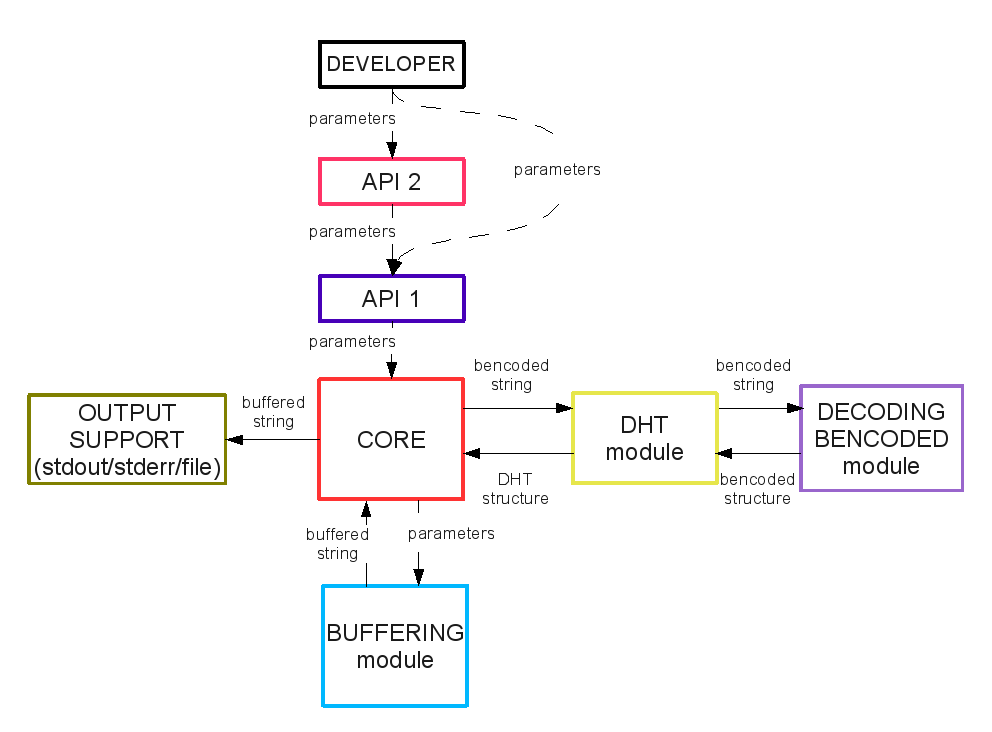
\includegraphics[width=0.7\textwidth]{src/img/proto-measure/log-library-architecture}
  \end{center}
  \caption{Monitoring with MonALISA}
  \label{fig:proto-measure:log-library-architecture}
\end{figure}

Next, parameters are sent to the core module that will verify and process
them. The core module may choose to pass some of the parameters to the DHT
module. If so, the DHT module will pass the same parameters to the decoding
bencoded strings module. The latter will create a bencoded structure that will
be passed back to the DHT module. Based on the received result, the DHT module
will create a DHT structure that will be also passed back to the core module.
The core will send all the prepared data to the buffering module which will
give in return a buffered string. Finally, the string will be printed out, for
standard output, standard error or a file.

\subsection{Library APIs}

The library provides two APIs that can be used by the developer. Designing the
library structure involved a trade-off between easing the use of library
functions and gaining all the message information supported by the BitTorrent
protocol.

In first phase, a set of API functions were developed considering only the
latter aspect. This phase of developing had as a main aim building an
interface that offers a true and valid functionality. It does not take into
consideration the peer state and information and that is why it can be
classified as a stateless API. The aim of the next phase represented the
making of a more developer-friendly interface. This was based on the first set
of functions from two reasons: first, allowing the programmer to use the first
set too if it stretches more easily on his/her implementation, and the second
one, the reuse of the code.

The second set of functions uses a structure that gathers the peer information
needed for logging such as peer address, peer client, torrent hash and name.
The structure is initialized when the client builds its own peer corresponding
structure. A reference to the structure representing the peer logging
information will be saved in the associated peer structure used by the client.
This approach is recommended because the first API functions needs a longer
list of arguments containing the peer parameters besides the particular
information provided by the BitTorrent message, while the second API uses for
the peer information only the reference to the corresponding peer logging
structure.

\subsection{Library Initialization and Cleanup}

The library provides initialization and exiting operations. At initialization,
the library saves the configuration parameters given as arguments at the
corresponding function call. The output configuration may be hard coded by the
programmer or set by the user via client's GUI. It may be a given format using
the list of output variables or a XML format. Also, the destination of the
output must be specified. It may be the standard output or the standard error,
or it may be a file. The destination may be specified using an environment
variable set with the name ``BTLOG'' or a string parameter given as argument at
initialization function call. The initialization supplies an extra option for
using a list of peers.

The developer may choose this option if he/she wants to leave the
responsibility of freeing the allocated memory necessary for peer structures
to the library's perspective. If the chosen API is the peer based one, then in
order to log message send to / received from  a peer, a structure
\texttt{peer\_log\_t} must be created prior to this. Also, in this case the
peer address will be passed using the structures provided by the Linux
platforms (\texttt{struct in\_addr} and \texttt{struct in6\_addr}). On each
call of the functions, the peer address will be converted to string by the
library.

When the client session ends, the library exit function must be called. If the
set output destination is a file, it is closed at the exit. Also, if the text
output format mode is set, the array of strings created by the core module for
printing the information is also cleared. In the case that the developer chose
to use the peer logging structures list provided by the library, the exit
function will release the memory allocated for them.

\subsection{Peer Logging Structure}

The \texttt{peer\_log\_t} structure is handled in a object oriented manner.
Variables of these type are created using a function as the constructor for
the object oriented classes. Modifications can be made using a set of
functions just as the setters are used in object oriented paradigm. This
approach spares the developer from allocating resources for data needed in
logging.

The \texttt{peer\_log\_t} instance should be created immediately after a
successful handshake is received. According to the protocol, the connection
between peers is established after the initiator of the handshake receives the
handshake message sent as response. The message contains the peer's identifier
and the SHA1 hash associated with the torrent. The IP and the port of the peer
must be known whenever a message will be sent or received on the TCP
connection. The name of the torrent  is known after the checking of the
\texttt{info\_hash} parameter of the handshake. If a peer sends a handshake,
it is implicitly admitted that it knows the torrent name. A handshake receiver
will get the torrent name after checking its availability in the client's list
of active torrents.

A \texttt{peer\_log\_t} instance may need modifications along the session from
different reasons. One reason may be if the client cannot complete the fields
of the structure immediately after the handshake message is sent or received.
This happens in two situations. First, if the processing of the handshake
involves an analysis of each parameter in different contexts. For example, if
different functions decode and verify each parameter, without saving or
passing it.  Second, if a protocol extension negotiation occurs and the
handshake is held on more steps. For connection encryption extension, the
steps involved follow the Diffie-Hellman key exchange protocol.

Another reason is if a ``port'' message is received. A ``port'' message is
sent by client versions that implement a DHT tracker. The listen port is the
port the peer's DHT node is listening on. Only then, the peer's port can be
set. When modifications must be brought to the \texttt{peer\_log\_t}
structure, the developer should use the setters provided by the logging
library.

The peer-state aware set of functions are build on the basic set of functions
of the first API. The \texttt{peer\_log\_t} reference variable given as
parameter is translated into the parameters used for calling the basic
functions.

The address of the peer will be translated into a string using the standard
representation. For IPv4 will be used the dotted decimal notation,
concatenated with a colon in front of the ASCII representation of the port.
For IPv6, will be used the hexadecimal notation inside brackets, concatenated
with a colon in front of the ASCII representation of the port.

\subsection{Core Module}

When a basic function of the first API is called, the arguments of the message
are sent to the core of the library. The library core is the part where the
message string is created. First of all, the core verifies the parameters
validity in order to assure a well formatted  and coherent message output
string. Depending on the parameters and the session state, the core decides on
how the printed message will look like. The string is buffered into an inner
library structure called \texttt{btl\_buffer\_t}. The message is composed of
different parts. For the text output mode, each part represents one of the
following:

\begin{itemize}
  \item \textbf{a format variable} -- one of the symbols of the format
  prefixed with the percent (`\%') character
  \item \textbf{a padding string} -- a component of the string, other than a
  format variable When a message component is created, it is added by the core
  to the buffer. Inside it, the buffer constructs the string containing the
  whole message, expanding its allocated memory size whenever is needed. All
  the format variables, excepting the \texttt{\%msg} variable will be printed
  in the same way for every message. The \texttt{\%msg} variable will be
  expanded in a different manner, depending on message specific
  characteristics.
\end{itemize}

The messages belonging to BitTorrent protocol, Fast Peers extension and
Connection Encryption extension are all treated the same. Excepting the
handshake message, the BitTorrent protocol message parameters are integer
values. They represent blocks coordinates relative to pieces indexes. The
handshake message has a string parameter which contains the protocol name and
eight reserved  bytes indicating the supported extensions of the initiating
client. The Fast Peers messages have also integer parameters corresponding to
the blocks being advertised. For the Connection Encryption, parameters are
rather few. Only the \texttt{crypto\_provide} and \texttt{crypto\_select}
messages have integer parameters which are printed for the output as
hexadecimal values, according to the extension specification.

An exceptional case is when Distributed Hash Table extension messages are sent
or received. Since DHT messages can have a significant number of parameters,
it would have been difficult not only to implement a different API function
for every type, but to use them too in BitTorrent client development. Thus,
the chosen solution was to create just two functions for incoming or outgoing
DHT messages, whose bencoded string is decoded in the library core. The
bencoded string is passed as argument by the developer. The core passes the
bencoded string to the DHT module that has the role of returning a DHT
structure based on the given encoded string. The DHT module calls the decoding
bencoded module who is able to analyze and verify the bencoded string. If the
string is well encoded, a bencoded structure is returned as response, else the
response is null.

\subsection{Buffering Module}

The message is buffered using the functions provided by the buffering module.
The buffering module has the role of creating a \texttt{btl\_buffer\_t}
structure which contains the characters that will be printed out. It provides
functions for adding new information depending on the output format type, text
or XML, and the parameter type. For each new add, the buffer is expanded if
the remained space is not enough for the information to be inserted.

After completing the buffer, the characters are written to the output
destination: standard output, standard error or the set file. After the
writing process ends, all the allocated resources are released.

\subsection{Output}

The logging output destination and format can be configured by both developer
or user to suit one's needs. The output can be redirected to standard output,
standard error or a set file, given as parameter. The format of the output can
be text mode, each line representing a message, or XML format, each message
representing a main node in XML tree structure. For a XML format, details
regarding the message are given in own tags.

\subsubsection{Text Mode}

When XML enabling parameter is omitted, the output format is considered. The
output format is a string that must contain the logging specific variables. A
logging specific variable is a variable from
Table~\ref{tab:proto-measure:liblog-variables} that has to be inserted in
format string in order to be printed. The variable will be expanded into its
corresponding value. All the other characters will be printed as they are
given in the format string, having the role of variables separators or
paddings.

\begin{table}[htb]
  \centering
  \caption{Library Logging Variables}
  \label{tab:proto-measure:liblog-variables}
  \begin{tabular}{@{}ll@{}}
    \toprule
      \textbf{Variable} & \textbf{Description} \\
    \midrule
      \texttt{\%time} & Time \\
      \texttt{\%address} & Peer address \\
      \texttt{\%client} & Peer client \\
      \texttt{\%torrname} & Torrent name \\
      \texttt{\%torrhash} & Torrent hash \\
      \texttt{\%inout} & Message direction \\
      \texttt{\%type} & Message type \\
      \texttt{\%msg} & Message content \\
    \bottomrule
  \end{tabular}
\end{table}

The format is processed at logging initialization and represented by an array
of strings, each string being associated with a format variable or a padding
string. When all the data for printing a message is available, the library
core browses the array in order to print its value. If an array element
represents a format variable, its corresponding logging data item will be
printed. Else, if it represents another string, the respective string will be
printed.

Each message is printed on a single line. Thus when the logging output will be
parsed, a read line-by-line approach will be fairly even. Example for a
``request'' message:

\begin{itemize}
  \item user provided format:
    \begin{verbatim}
[%time] %address <%client> "%torrname" (%inout) %type: %msg
    \end{verbatim}
  \item library output:
    \begin{verbatim}
[15:54:47.287] 24.132.173.70:54404 <µTorrent 1.8.1> "Ubuntu_8.10"
(Send) Request: index=1532 offset=262144 size=16384
    \end{verbatim}
\end{itemize}

As we can see, the time is shown between brackets, the address has the IPv4
standard representation, the peer's client name is ``µTorrent 1.8.1'' and the
torrent name is ``Ubuntu\_8.10''. The message is being sent, just as the
\textit{Send} label indicates, and message contains the index of the piece
that has the requested block, the offset of the block inside the piece and the
block size.  The output respects the given format as it is.

\subsubsection{XML Mode}

The XML output file contains an well-formed tree-based information. Messages
are logged as XML elements, each message argument being represented as a
nested element. The arguments order is hard coded, thus it cannot be configured
or reorganized.

The XML format was properly chosen so that output analysis and parsing could
be easily processed. The output is well-formed and easy to read. Messages have
a clear structure, each argument being constructed as  a XML element. The
message parameters are gathered in a XML \texttt{params} element. Depending on
the message specific data, message elements may vary.

The root element is named \texttt{btlog} and holds as attributes the starting
date and time, and the logging client name. Each message is represented by an
\texttt{message} element nesting the arguments. Arguments are also XML
elements, each one being named after the argument itself. The SHA1 20-byte
hashes are printed as 40-hexadecimal digits, 2 digits per hashing byte. A
printed  message may look like this:

\lstset{language=XML,caption=XML Output
Message,label=lst:proto-measure:xml-message}
\begin{lstlisting}
<message type="KeepAlive">
    <time>15:42:33.736</time>
    <address>82.121.44.31:22831</address>
    <client>"Transmission 1.71"</client>
    <torrent_name>"Ubuntu 8.10"</torrent_name>
    <torrent_hash>3132333435363738393031323334353637383930</torrent_hash>
    <dir>Send</dir>
    <params>
    </params>
</message>
\end{lstlisting}

As we can see in the example above, a \texttt{KeepAlive} message has no
parameters as it is specified in the BitTorrent protocol. Time is expressed in
hours, minutes, seconds and milliseconds. The address is a concatenation
between the standard IPv4 representation, colon separator and the TCP port.
IPv6 are also supported. The \texttt{dir} element may contain the values
\texttt{Send} or \texttt{Got}, determining message direction.

The \texttt{params} element nests the message specific parameters, which are
included in the BitTorrent message payload. For example, for a request message
the parameters are printed like this:

\lstset{language=XML,caption=params Element in XML Output
Message,label=lst:proto-measure:xml-params}
\begin{lstlisting}
<params>
    <index>49</index>
    <begin>12</begin>
    <length>1002</length>
</params>
\end{lstlisting}

\texttt{index} indicates the piece containing the requested block,
\texttt{begin} -- its piece offset, and \texttt{length} -- its block size.

\subsection{Clients Instrumented to Use the Library}

The library design aim was to cover an wide range of BitTorrent clients needs.
Inserting API functions into existent BitTorrent clients source code may be a
difficult task. That is why the library provides functions that can help the
developer to adjust the stored items such as peer information or  message
arguments to library demands. As long as a developer does not include a
detailed code specification or enough comments, it is difficult for a third
party developer to modify the whole code so that all the exchanged messages to
be captured.

There are a few wide used BitTorrent libraries: libtorrent rakshasa,
libtorrent rasterbar, MonoTorrent and BTSharp. Excepting the latter, the rest
of them are released under open source license. They are not used by a vast
majority of clients. Some of the clients are not keen on saving information in
order to be logged later. The two library APIs provide sufficient functions
for a good functionality. This does not necessarily imply developing
convenience because it depends on the client implementation.

In order to provide a valuable use of the library, we updated two such
instances: the \textit{libtransmission} component of the Transmission client
and \textit{libtorrent-rakshasa}, linked against the rtorrent client.

\subsubsection{rtorrent}

rTorrent is a C++ client written by Jari Sundell and it uses as back end the
free (under GNU GPL) libtorrent-rakshasa
library\footnote{http://libtorrent.rakshasa.no/}. The rakshasa library does
not logs the messages exchanged, it only outputs error messages for debugging.
For testing the btlog library, modifications to the rakshasa library were
required.

The modified files of the libtorrent library are in \texttt{src/} directory.
It is initialized in the initialize function from the
\texttt{torrent/torrent.cc} file. For setting the btlog library, a wrapper
function was created as seen in
Listing~\ref{lst:proto-measure:liblog-init-rakshasa}.

\lstset{language=C,caption=Initializing Logging Library for
libtorrent-rakshasa,label=lst:proto-measure:liblog-init-rakshasa}
\begin{lstlisting}
static void btlogInitialization(void)
{
    const char * format = NULL;
    const char * xml_env = getenv("XML_ENABLED");
    int xml_enabled = 0;

    if(xml_env)
        xml_enabled = atoi(xml_env);
    else
        format = getenv("BTLOG_FORMAT");

    btlogInit(PACKAGE_STRING, 1, format, xml_enabled);
}
\end{lstlisting}

The output format is given by the \texttt{BTLOG\_FORMAT} environment variable.
The enabling XML output flag is also set as a \texttt{XML\_ENABLED}
environment variable. If XML is enabled, then the text format it is not
passed, nor read.

Rakshasa uses a \texttt{PeerInfo} class for every peer that it exchanges
messages with.  The peer logging structure reference was linked as a field of
this class. When an object of this class is instantiated then the peer logging
structure is also created, but only by setting the address and the port. The
other fields are set at the handshake successfully end. This is done in the
insert function from \texttt{torrent/peer/connection\_list.cc}. The wrapper
used for setting the other fields is shown in
Listing~\ref{lst:proto-measure:liblog-rakshasa}

\lstset{language=C,caption=Library Logging in
libtorrent-rakshasa,label=lst:proto-measure:liblog-rakshasa}
\begin{lstlisting}
void initPeerLog(PeerInfo * peerInfo, DownloadInfo * downloadInfo)
{
    const char * peer_id = peerInfo->id().c_str();
    const char * name = downloadInfo->name().c_str();
    const char * hash = downloadInfo->hash().c_str();
    char torrHash[HASH_SIZE];

    memset(torrHash, 0, HASH_SIZE);
    memcpy(torrHash, hash, HASH_SIZE);

    if(!peerInfo->peer_log)
        peerInfo->peer_log = newPeerLog(peerInfo->socket_address(),
                                          peerInfo->listen_port(),
                                          peer_id, name, torrHash);
    else {
        logSetPeerClientFromId(peerInfo->peer_log,
                                 peerInfo->id().c_str());
        logSetPeerTorrName(peerInfo->peer_log, name);
        logSetPeerTorrHash(peerInfo->peer_log, torrHash);
    }
}
\end{lstlisting}

The \texttt{PeerInfo} class saves the peer ID, while the \texttt{DownloadInfo}
class contains the torrent hash and name. The peer ID is translated by the
library in a human readable client name.

\subsubsection{Transmission}

Transmission\footnote{http://www.transmissionbt.com/} is a BitTorrent client
written in C. It has its own BitTorrent library called
\textit{libtransmission}. It was the first tested client for the logging
library and it influenced the first implementation changes. Transmission
already has a strong logging system, but most of the logged data contains
information on inner events. Thus, the logging files have enormous dimensions,
while the logging library output contains only information regarding the
BitTorrent protocol.

The logging library is used by the Transmission client as a bundled static
library. Its sources are saved in the third-party directory and are compiled
once with the other third-party used modules. This was possible by adding a
Makefile.am file for the automake tool which is used for automated client
compilation. It contains the file names of the library and the built library
name: libbtlog.a. Library initialization is made in the
\texttt{tr\_sessionInit}
function of the \texttt{session.c} source file. The peer logging structure reference
(\texttt{peer\_log\_t}) was hooked in the \texttt{tr\_peerIo} structure of the
client, which is used for every event regarding a valid connection with a
peer. The peer logging structure is initialized in the \texttt{tr\_peerIoNew}
function from \texttt{peer-io.c} as described in
Listing~\ref{lst:proto-measure:liblog-transmission}.

\lstset{language=C,caption=Library Logging in
Transmission,label=lst:proto-measure:liblog-transmission}
\begin{lstlisting}
static tr_peerIo * tr_peerIoNew(...,
                                const tr_address * addr,
                                tr_port            port,
                                const uint8_t    * torrentHash,
                                ...)
{
    tr_peerIo * io;

    ...

    /* BTLOG create peer log */
    if( addr->type == TR_AF_INET )
        io->peer_log = newPeerLogV4(&addr->addr.addr4, port, 
                                  NULL, NULL, torrentHash);
    else
        io->peer_log = newPeerLogV6(&addr->addr.addr6, port,
                                  NULL, NULL, torrentHash);

    ...
}
\end{lstlisting}

Only the address, the port and the torrent hash are known when the structure
is created. The other fields are completed using the setter functions in
further contexts. Transmission processes the client and the torrent names
merely after the handshake is successful. This is done by the
\texttt{myHandshakeDoneCB} function of the \texttt{peer-mgr.c} source file.
The API message logging functions are called in the \texttt{peer-msgs.c}
source file functions.

\section{Log Collecting for BitTorrent Peers}
\label{sec:proto-measure:log-collect}

The log collection approach implying a less intrusive activity but providing a
great deal of protocol parameters is the use of logging information from
clients. Each client typically presents a status information (the dubbed
\textit{status message}) consisting of periodic information such as download
speed, upload speed, number of connection and, if enabled, a set of enhanced
pieces of information (the dubbed \textit{verbose message}). Types of messages
and their content have been thoroughly described in
Section~\ref{sec:proto-measure:protocol-messages}. All or most of BitTorrent
clients provide status messages but some sort of activation or instrumentation
is required to provide verbose messages.

\subsection{Using and Updating BitTorrent Clients for Logging}

Throughout experiments we have used multiple open-source clients. All of them
provided basic status information, while some were updated or altered to
provide verbose information as well. Transmission, Aria2, Vuze, Tribler,
libtorrent-rasterbar and the mainline client had been used to provide status
parameters, while Tribler and libtorrent-rasterbar had also been instrumented
to provide verbose parameters.

Several approaches had been put to use to collect status information,
depending on the client implementation:

\begin{itemize}

  \item The main issue with \textbf{Azureus} was the lack of a proper CLI that
  would enable automation. Though limited, a ``Console UI'' module enabled
  automating the tasks of running Azureus and gathering download status and
  logging information.

  \item Although a GUI oriented client, \textbf{Tribler} does offer a command
  line interface for automation.

  \item \textbf{Transmission} has a fully featured CLI and was one of the
  clients that were very easy to automate. Detailed debugging information
  regarding connections and chunk transfers can be enabled by setting the
  \texttt{TR\_DEBUG\_FD} evironment variable.

  \item \textbf{aria2} natively provides a CLI and it was easy to automate.
  Logging is also enabled through CLI arguments.

  \item \textbf{hrktorrent} is a lightweight implementation over
  \textbf{libtorrent-rasterbar} and provides the necessary interface for
  automating a BitTorrent transfer, albeit some minor modifications have been
  necessary.

  \item \textbf{BitTorrent Mainline} provides a CLI and logging can be enabled
  through minor modifications of the source code.

\end{itemize}


In order to examine BitTorrent transfer parameters at a protocol
implementation level, we propose a system for storing and analysing logging
data output by BitTorrent clients. It currently offers support for
hrktorrent/libtorrent\footnote{http://www.rasterbar.com/products/libtorrent/}
and Tribler\footnote{http://www.tribler.org/trac}.

Our study of logging data takes into consideration two open-source BitTorrent
applications: Tribler and hrktorrent\footnote{http://50hz.ws/hrktorrent/}
(based on libtorrent-rasterbar. While the latter needed minimal changes in
order to provide the necessary verbose and status data, Tribler had to be
modified significantly.

The process of configuring Tribler for logging output is completely automated
using shell scripts and may be reversed. The source code alterations are
focused on providing both status and verbose messages as client output
information.

\textit{Status message} information provided by Tribler includes transfer
completion percentage, download and upload rates. In the modified version, it
also outputs current date and time, transfer size, estimated time of arrival
(ETA), number of peers, and the name and path of the transferred file.

In order to enable \textit{verbose message} output, we took advantage of the
fact that Tribler uses flags that can trigger printing to standard output for
various implementation details, among which are the actions related to
receiving and sending BitTorrent messages. The files we identified to be
responsible for protocol data are changed using scripts in order to print the
necessary information and to associate it to a timestamp and date. Since most
of the protocol exchange data was passed through several levels in Tribler's
class hierarchy, attention had to be paid to avoid duplicate output and to
reduce file size. In contrast to libtorrent-rasterbar, which, at each transfer,
creates a separate session log file for each peer, Tribler stores verbose
messages in a single file. This file is passed to the verbose parser, which
extracts relevant parts of the messages and writes them into the database.

Unlike Tribler, hrktorrent's instrumentation did not imply modifying its
source code but defining \texttt{TORRENT\_LOGGING} and
\texttt{TORRENT\_VERBOSE\_LOGGING} macros before building (recompiling)
libtorrent-rasterbar. Minor updates had to be delivered to the compile options
of hrktorrent in order to enable logging output.

Although our system processes and stores all protocol message types,
the most important messages for our swarm analysis are those related to
changing a peer's state (choke/unchoke) and requesting/receiving data.
Correlations between these messages are the heart of provisioning information
about the peers' behaviour and BitTorrent clients' performance.

\subsection{Storage}

Logging information is typically stored in log files. In
libtorrent-rasterbar's case, logging is using a whole folder and logging
information for each remote peer is using a single file in that folder.
Usually information is redirected from standard output and error towards the
output file.

As in a given experiment, logging information occupies a large portion of
disk space, especially verbose messages, files and folders are compressed in
archive files. There would generally be a log archive for each client session.
When information is to be processed, logging archives are going to be provided
to the data processing component. A log archive contains both status messages
and verbose messages.

Logging information may be stored in archive files for subsequent use or it
may be processed live -- that is parsing and interpreting parameters as log
files are being generated. When running a live/real-time processing component,
compressing logging information may not be required. However, in order to
still preserve the original files, some experimenters may choose to retain
access to the log archives.

The usefulness of a live processing component is based primarily on
relieving the burden of space consumption, in case archiving is disabled. Most
of the logged information is not useful, due to the fact that some peers may
not be connected to other peers and status information, though provided,
consists of parameters that are equal to zero -- no connections means
\texttt{0 KB/s} download speed, \texttt{0 KB/s} upload speed and others. On a
certain occasion, a log file that had been used for more than 3 weeks,
occupied more than 1GB of data but resulted in just 27KB valuable
information.

Either when using live parsers or subsequent analysis, parameters are parsed
for rapid use. The post-parsing storage is typically a relational database.
The advantage of such a storage facility is its rapid access for
post processing. When inquiring about given swarm parameters, the user would
query the database and rapidly obtain necessary information. If that wouldn't
be enabled, each inquiry would require a new parsing activity, resulting in
large overhead and CPU consumption. Database storage is the final step of the
logging and parsing stage. Parameter analysis, interpretation and advising
activities would not be concerned of logging information, but only query the
database.

\subsection{Experiments}

In order to collect information specific to a swarm, one must have access to
all clients and logging information from those clients. As such, either all
clients are accessible to the experimenter, or users would subsequently
provide logging information to the experimenter.

Some remote information may be replaced by that provided by a tracker log
file. A tracker logs information regarding the overall swarm view, albeit its
periodicity is quite large (typically 30 minutes -- 1800 seconds).

An intermediate approach to collecting logging information is a form of
aggregation of information on the client side. This information may be either
sent to a logging service or stored to be subsequently provided to the user.
The former approach it taken by the Logging Service withing the P2P-Next
project.

Typical experiments are those that allow full control to the user and provide
all information rendered by clients. These experiments are using the
virtualization infrastructure described in Chapter~\ref{chapter:virt-infra}.
Deployment, log activation, log collection/archiving and even parsing are
accomplished in full automation. One would create a configuration file and run
experiments. Log archive files typically result from the experiment and, after
gathering all, may be subjected to analysis.

The inclusion of tracker information had been enabled in the use of UPB Linux
Distro Experiments\footnote{http://torrent.cs.pub.ro/}. Tracker log files are
parsed live and provide overall swarm parameters. Various information from
tracker log files are provided as graphic images that show the evolution of
swarm parameters.

Tracker logs have also been enabled in Living Lab experiments as described in
Section~\ref{subsec:multimedia-dist:nextshare-ll}. These experiments rely on
extensive logging information (verbose messages) provided by seeders and
tracker information. The lack of complete access to the all clients in the
swarm is balanced out by the usage of verbose logging on the seeders' side.
However, remote peers' intercommunication is not logged in anyway. Such that a
form of aggregation and collection of remote peers' intercommunication
messages is still required.

\subsection{Monitoring and Post-Processing}

Log processing, as described in
Section~\ref{sec:proto-measure:data-processing} refers to parsing and
interpreting BitTorrent protocol parameters. Data is parsed into an easy to be
accessed database that is provided to the user.

As described above, one may choose to store logging information and then
enable analysis. We dub this approach \textit{post-processing}. The other
approach is for live analysis of the provided parameters, resulting in client
and swarm monitoring. The two approaches may, of course be combined: while
doing parsing of information, it is also stored in a database while various
parameters are also monitored.

An overview of a typical architecture for data processing is presented in
Figure~\ref{fig:proto-measure:ppf-architecture}. Separate parsers are used for live parsing and
classical parsing. Classical parsing results in a database ``output'', while
live parsing results in both a database ``output'' and the possibility of
deploying live client and swarm monitoring.

\section{Protocol Data Processing Engine}
\label{sec:proto-measure:data-processing}

As client instrumentation provides in-depth information on client
implementation, it generates extensive input for data analysis. Coupled
with carefully crafted experiments and message filtering, this will allow
the detection of weak spots and of improvement possibilities in current
implementations. Thus it will provide feedback to client and protocol
implementations and swarm ``tuning'' suggestions, which in turn will enable
high performance swarms and rapid content delivery in peer-to-peer systems.

Due to various types of modules employed (such as parser implementations,
storage types, rendering engines) a data processing framework may provide
different architectures. A sample view of the infrastructure consists of the
following modules:

\begin{itemize}
  \item \textbf{Parsers} -- receive log files provided by BitTorrent
clients during file transfers. Due to differences between log file formats,
there are separate pairs of parsers for each client. Each pair analyses status
and verbose messages.
  \item \textbf{Database Access} -- a thin layer between the database system and
other modules. Provides support for storing messages, updating and reading
them.
  \item \textbf{SQLite Database} -- contains a database schema with tables
designed for storing protocol messages content and peer information.
  \item \textbf{Rendering Engine} -- consists of a GUI application that
processes the information stored in the database and renders it using plots
and other graphical tools.
\end{itemize}

\begin{figure}[h]
  \begin{center}
    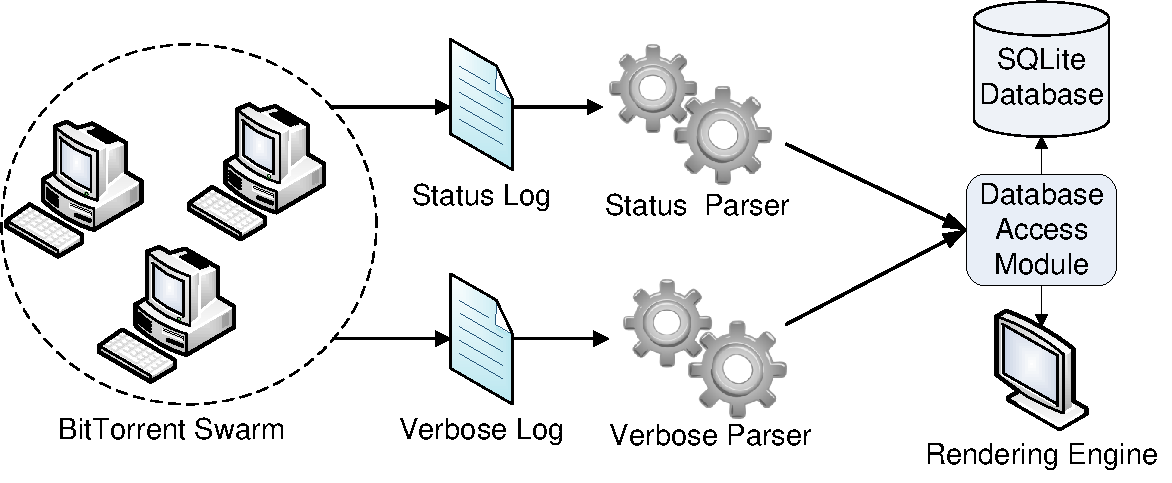
\includegraphics[width=0.7\textwidth]{src/img/proto-measure/logarch-not-use}
  \end{center}
  \caption{Logging System Overview}
  \label{fig:proto-measure:logarch}
\end{figure}

As shown in Figure~\ref{fig:proto-measure:logarch}, using parsers specific to
each type of logging file, messages are sent as input to the \textit{Database
Access} module that stores them into an SQLite database. In order to analyse
peer behaviour the \textit{Rendering Engine} reads stored logging data using
the \textit{Database Access} module and outputs it to a graphical user
interface.

Once all logging and verbose data from a given experiment is collected, the
next step is the analysis phase. The testing infrastructure provides a GUI
(\textit{Graphical User Interface}) statistics engine for inspecting peer
behaviour.

The GUI is implemented in Python using two libraries: \textit{matplotlib}
-- for generating graphs and \textit{TraitsUi} -- for handling widgets. It
offers several important plotting options for describing peer behaviour and
peer interaction during the experiment:

\begin{itemize}
  \item \textit{download/upload speed} -- displays the evolution of
download/upload speed for the peer;
  \item \textit{acceleration} -- shows how fast the download/upload speed of
the peer increases/decreases;
  \item \textit{statistics} -- displays the types and amount of verbose
messages the peer exchanged with other peers.
\end{itemize}

The last two options are important as they provide valuable information about
the performance of the BitTorrent client and how this performance is
influenced by protocol messages exchanged by the client.

A sample GUI screenshot may be observed in
Figure~\ref{fig:proto-measure:processing-gui-1} and
Figure~\ref{fig:proto-measure:processing-gui-2}

\begin{figure}[h]
  \begin{center}
    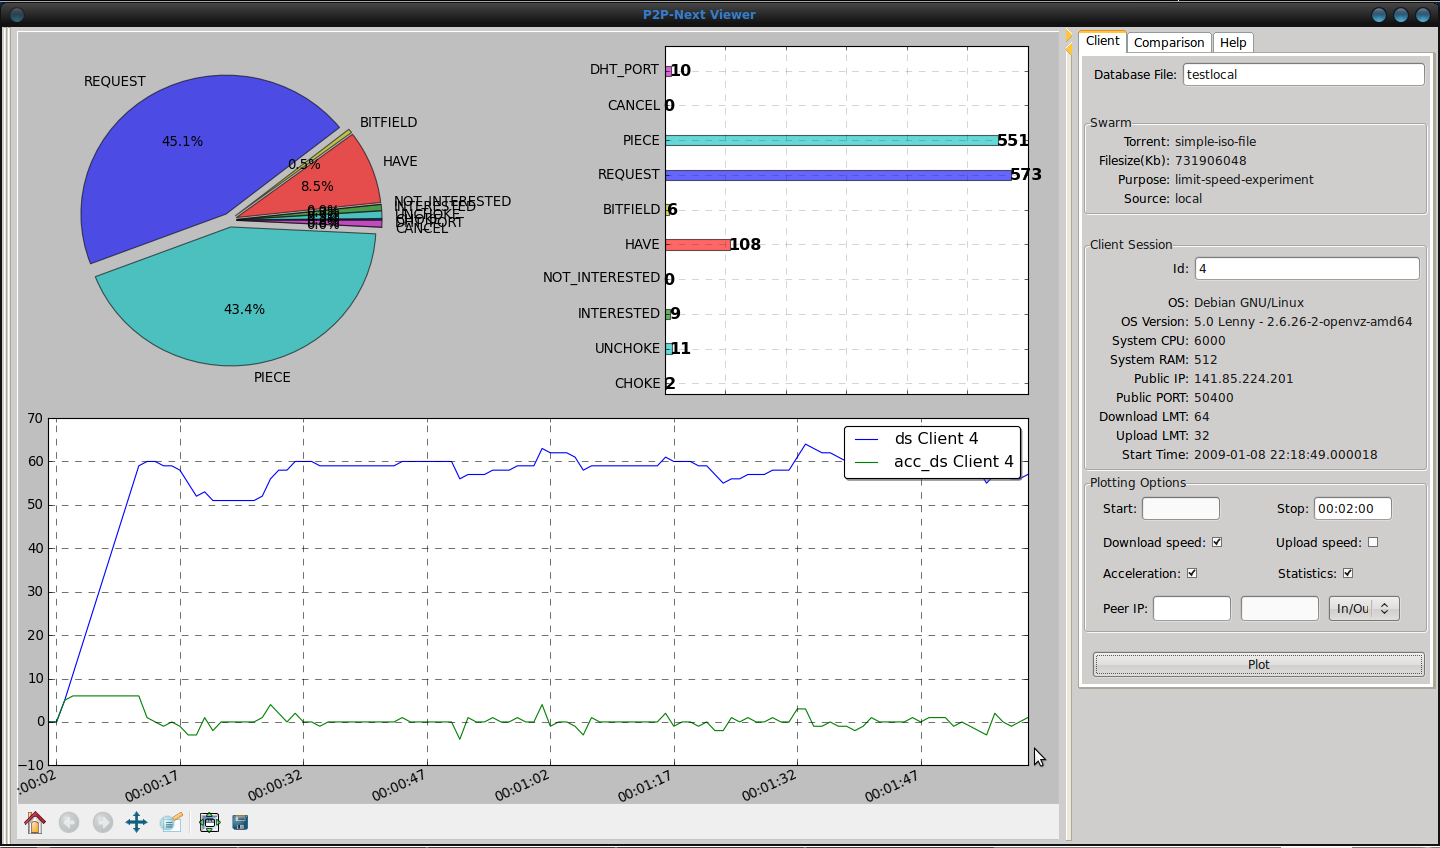
\includegraphics[width=0.7\textwidth]{src/img/proto-measure/processing-gui-1}
  \end{center}
  \caption{Rendering Engine for BitTorrent Parameters: Client Analysis}
  \label{fig:proto-measure:processing-gui-1}
\end{figure}

\begin{figure}[h]
  \begin{center}
    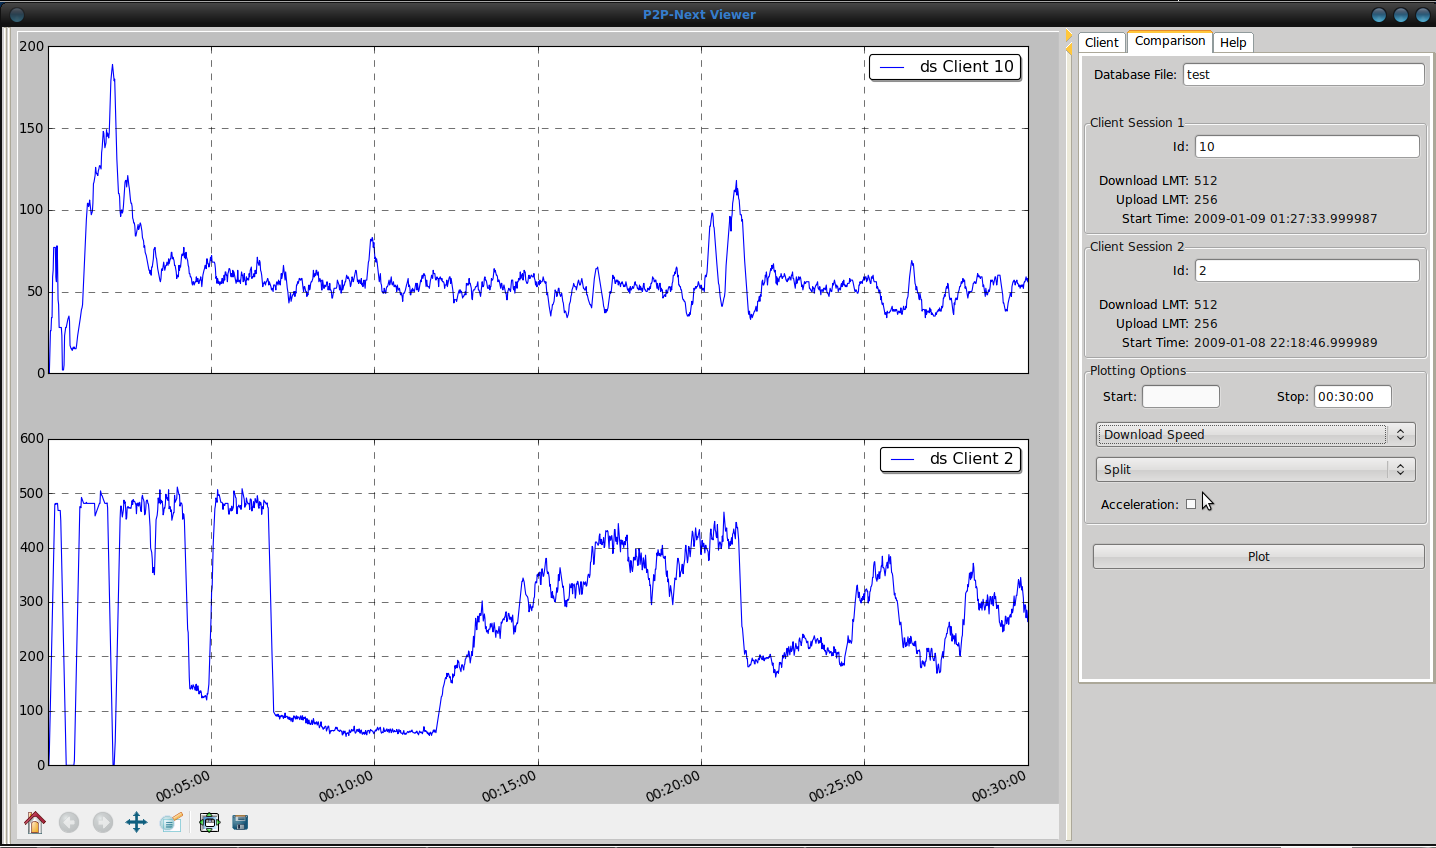
\includegraphics[width=0.7\textwidth]{src/img/proto-measure/processing-gui-2}
  \end{center}
  \caption{Rendering Engine for BitTorrent Parameters: Client Comparison}
  \label{fig:proto-measure:processing-gui-2}
\end{figure}

The \textit{acceleration} option measures how fast a BitTorrent client is able
to download data. High acceleration forms a basic requirement in live
streaming, as it means starting playback of a torrent file with little delay.

The \textit{statistics} option displays the flow of protocol messages. We are
interested in the choke/unchoke messages.

The GUI also offers two modes of operation: \textit{Single Client Mode},
in which the user can follow the behaviour of a single peer during a given
experiment, and \textit{Client Comparison Mode}, allowing for comparisons
between two peers.

\subsection{Post Processing Framework for Real-Time Log Analysis}

The dubbed post processing framework is used for storing logging information
provided by various BitTorrent clients into a storage area (commonly a
database). An architectural view of the framework is described in
Figure~\ref{fig:proto-measure:ppf-architecture}.

\begin{figure}[h]
  \begin{center}
    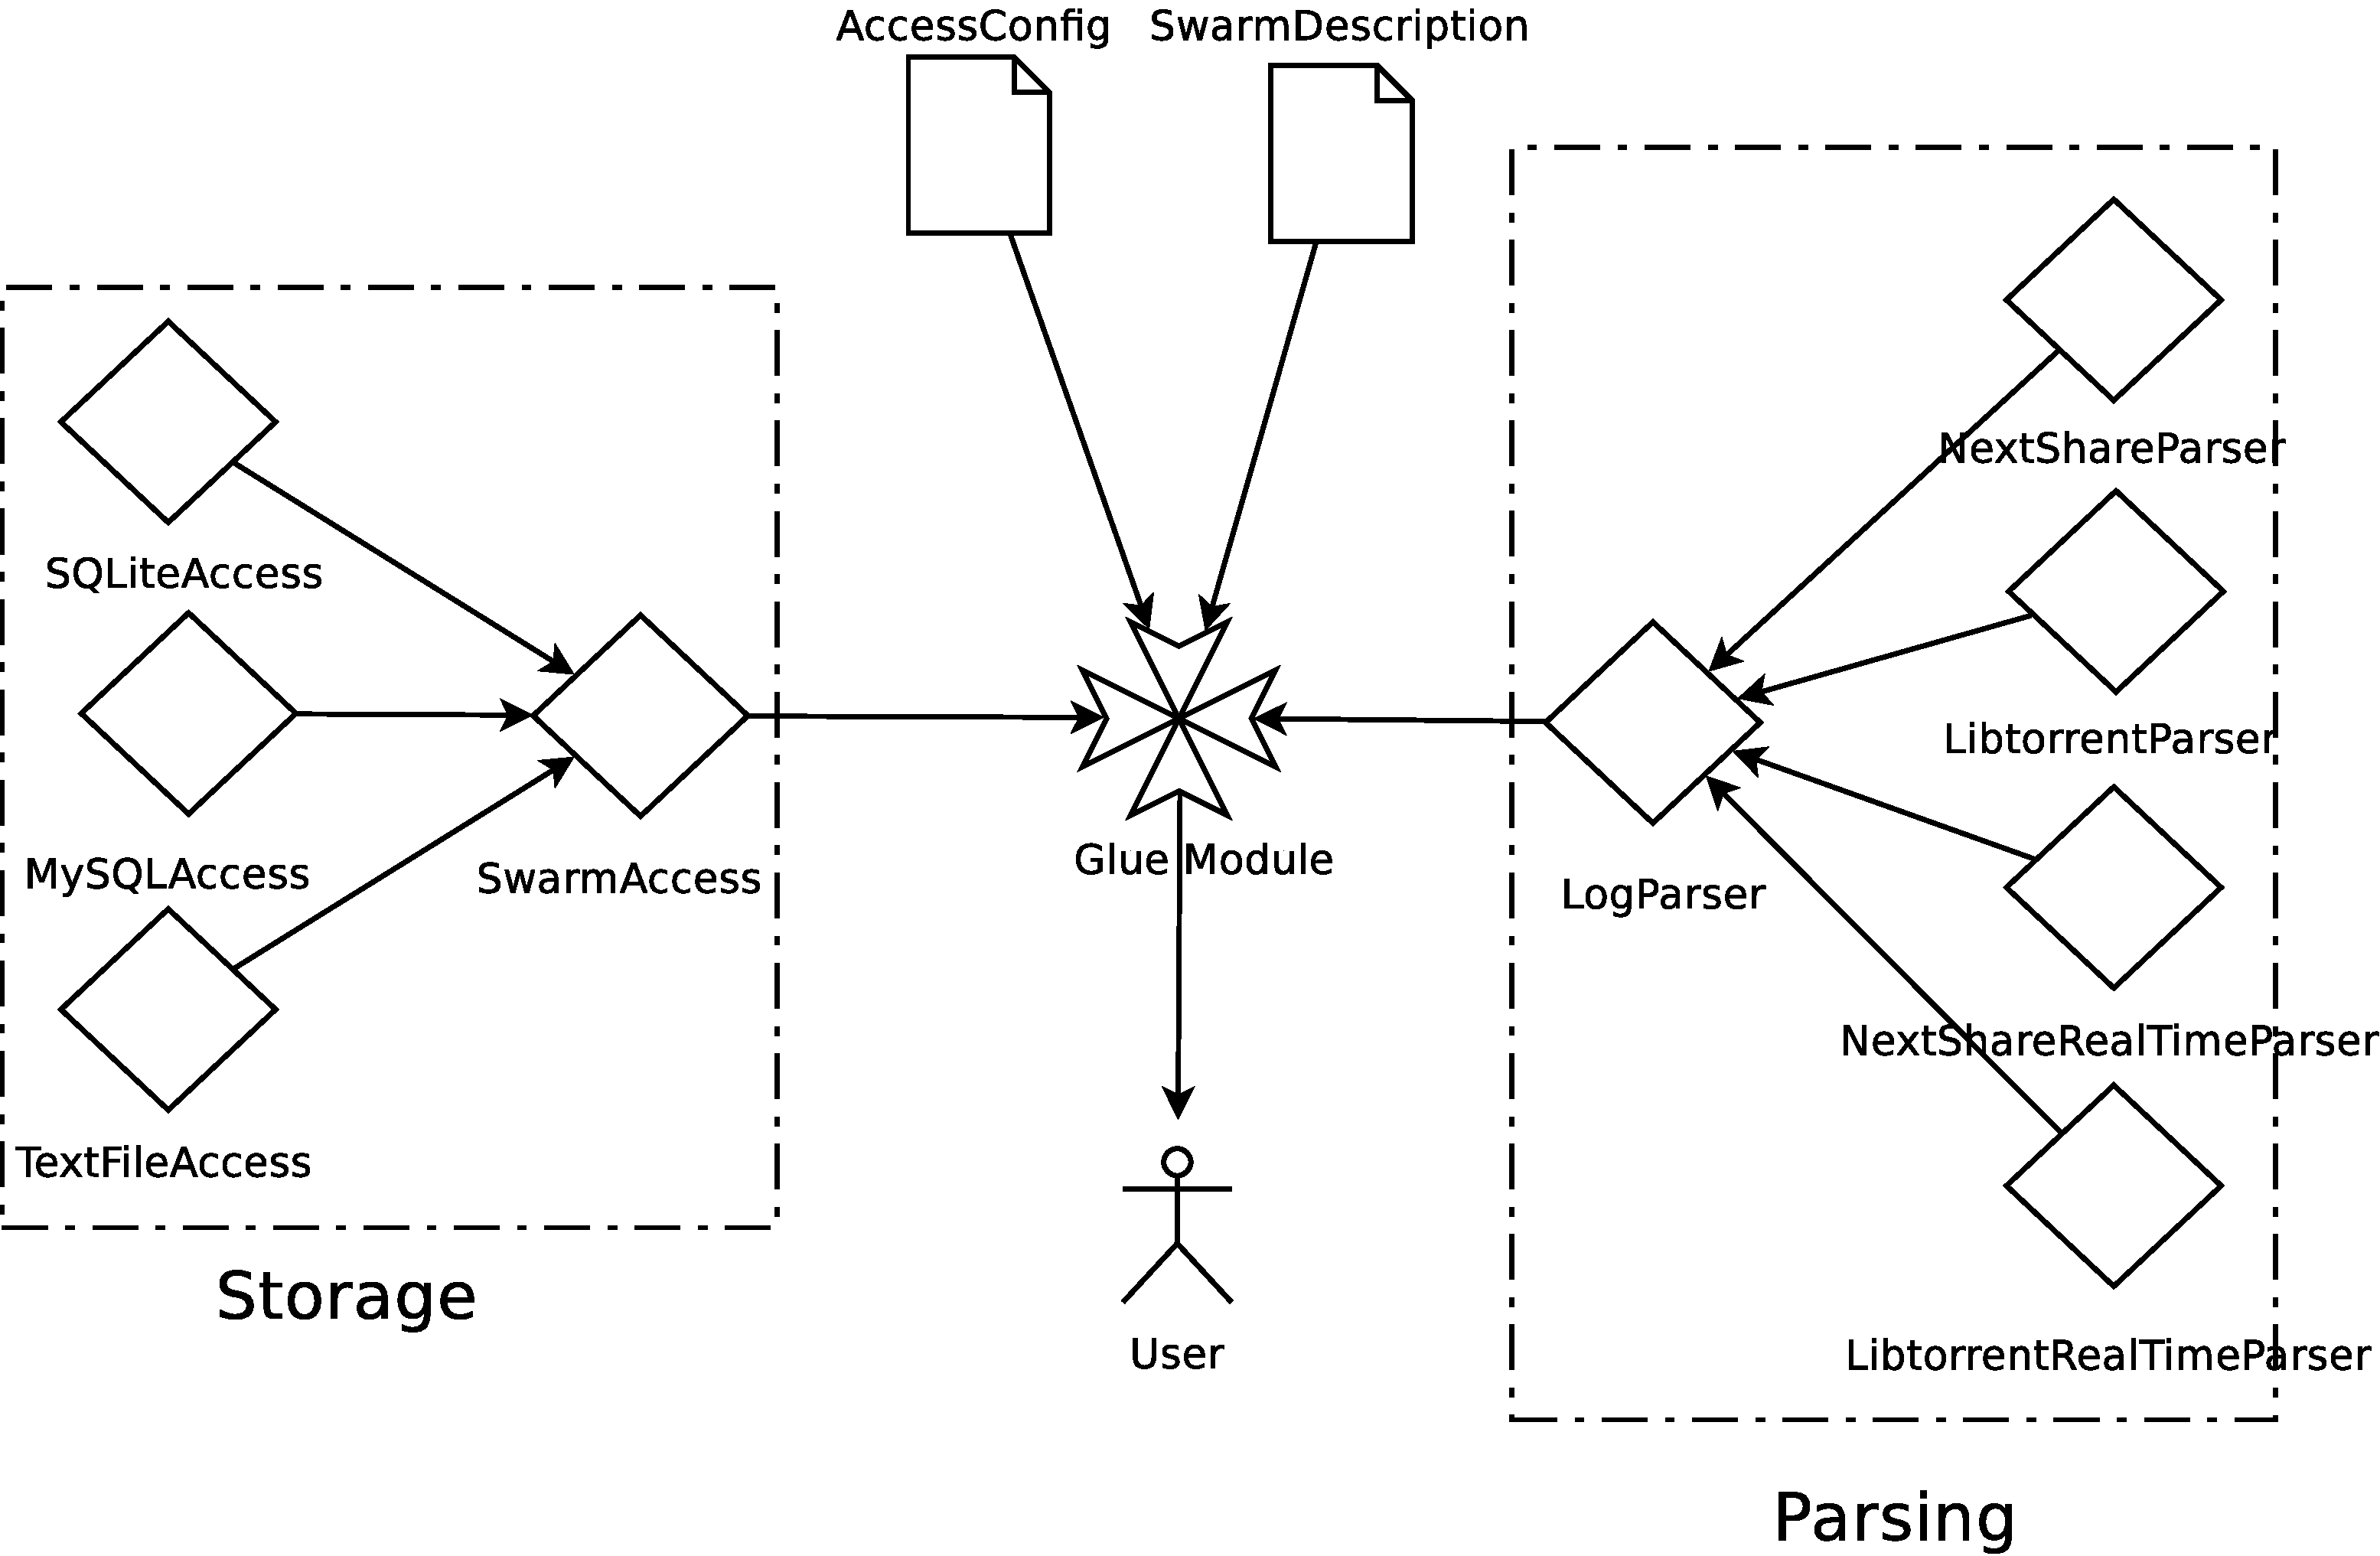
\includegraphics[width=0.7\textwidth]{src/img/proto-measure/ppf-architecture}
  \end{center}
  \caption{Post-Processing Framework Architecture}
  \label{fig:proto-measure:ppf-architecture}
\end{figure}

The two main components of the framework are the parser and the storage
components. Parsers process log information and extract measured protocol
parameters to be subject to analysis; storers provide an interface for
database or file storing -- both for writing and reading. Storers thus provide
an easy to access, rapid to retrieve and extensible interface to parameters.
Storers are invoked when parsing messages -- for storing parameters, and when
analyzing parameters -- for retrieving/reading/accessing parameters.

Within the parser component, a \texttt{LogParser} module provides the
interface to actual parser implementations. There are two kinds of parsers:
log parsers and real time log parsers. The former are used for data already
collected and subsequently provided by the experimenter. Another approach
involves using parsers at the same time as the client generates logging
information. This real time parsing approach possesses three important
advantages: monitoring may be enabled for status messages, less space is
wasted as messages are parsed in real time, and processing time is reduced due
to the overlapping of the parsing time and the storing time. The disadvantage
of a real time parser is a more complex implementation as it has to consider
the current position in the log file and continue from that point when data is
available. At the same time, all clients must be able to access the same
database, probably located on a single remote system.

The storage component is interfaced by the \texttt{SwarmAccess} module. This
module is backed by database-specific implementations. This may be RDMBS
systems such as MySQL or SQLite or file-based storage. Parameters are stored
according to the schema described in
Figure~\ref{fig:proto-measure:database-schema}.

Configuration of the log files and clients to be parsed is found in the
\textit{SwarmDescription} file. All data regarding the current running swarm
is stored in this file. Client types in the description file also determines
the parser to be used. Selection of the storage module is based on the
configuration directives in the \textit{AccessConfig} file. For an SQLite
storage, this contains the path to the database file; for an MySQL file, it
contains the username, password, database name common to database connection
inquiries.

The user/developer is interfaced by a \textit{Glue Module} that provides all
methods deemed necessary. The user would call methods in the Glue Module for
such actions as parsing a session archive, a swarm archive, for updating a
configuration file, for retrieving data that fills a given role.

\subsubsection{Parameter Storage Database}

The database schema as shown in Figure~\ref{fig:proto-measure:database-schema}
is used for relational database engines such as MySQL or SQLite.

\begin{figure}[h]
  \begin{center}
    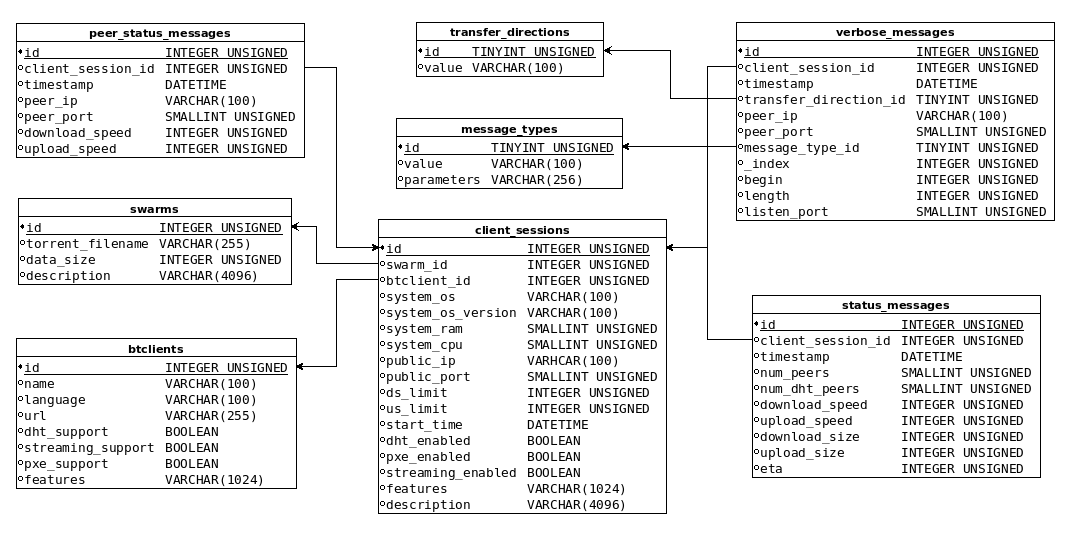
\includegraphics[width=0.7\textwidth]{src/img/proto-measure/database-schema}
  \end{center}
  \caption{Database Schema}
  \label{fig:proto-measure:database-schema}
\end{figure}

The database schema provides the means to efficiently store and rapidly
retrieve BitTorrent protocol parameters from log messages. The database is
designed to store parameters about multiple swarms in the \texttt{swarms}
table; each swarm is identified by the \texttt{.torrent} file its clients are
using.

Information about peers/clients that are part of the swarm are stored in the
\texttt{client\_sessions} table. Each client is identified by its IP address
and port number. Multiple pieces of information such as BitTorrent clients in
use, enabled features and hardware specifics are also stored.

Three classes of messages result in three tables:
\texttt{status\_messages}, \texttt{peer\_status\_messages} and
\texttt{verbose\_messages}. The \texttt{peer\_status\_messages} table stores
parameters particular to remote peers connected to the current client, while
the \texttt{status\_messages} stores parameters specific to the current client
(such as download speed, upload speed and others). Each line in the
\texttt{*\_messages} tables points to an entry in the
\texttt{client\_sessions} table, identifying the peer it belongs -- the one
that generated the log message.

\subsubsection{Logfile-ID Mapping}

When parsing log files, one has to know the ID of the client session that has
generated the log file. In order to automate the process, there needs to be a
mapping between the log file (or log archive) and the client session ID.

At the same time, the client session ID needs to exist in the
\texttt{client\_sessions} table in the database, together with information
such as BitTorrent client type, download speed limitation, operating system,
hardware specification etc. This information needs to be supplied by the
experimenter in a form that is both easy to create (by the experimenter) and
parse.

A swarm description file is to be supplied by the experimenter. This file
consists all required swarm and peer information including the name/location
of the log file/archive.

As we consider the INI format to be best suited for this, as it is fairly easy
to create, edit and update, it was chosen to populate initial information. The
experimenter may easily create an INI swarm description file and provide it to
the parser together with the (compressed) log files.

The swarm description file is to be parsed by the experimenter and SQL queries
will populate the database. One entry would go into the \texttt{swarms} table
and a number of entries equal to the number of peers in the swarm description
file would go into the \texttt{client\_sessions} table. As result of these
queries, swarm IDs and client sessions IDs are going to be created when
running SQL insert queries (due to the \texttt{AUTO\_INCREMENT} options). This
IDs are essential for the message parsing process and are going to be written
down in the Logfile-ID-Mapping-File.

The swarm description file parser is going to parse that file and also generate a logfile-id mapping file. The parser is responsible for three actions:
\begin{itemize}
  \item parsing the swarm description file
  \item creating and running SQL insert queries in the \texttt{swarms} and
  \texttt{client\_sessions} tables
  \item create a logfile-id mapping file consisting of mappings between client
  session IDs and log/file
\end{itemize}

A logfile-id mapping file is to be generated by the swarm description parser
and will subsequently be used by the message parser (be it status messages or
verbose messages). The mapping file simply maps a client session ID to a log
file or a compressed set of log files. A sample file is stored in the
repository (source:ppf/log-samples/log-id-mapping/log-id-mapping.sample.ini).
The message parser doesn't need to know client session information; it would
just use the mapping file and populate entries in the \texttt{*\_messages}
tables.

The message parser is going to use the logfile-id mapping file and the log
file (or compressed set of log files) to populate the \texttt{*\_messages}
tables in the database (\texttt{status\_messages},
\texttt{peer\_status\_messages}, \texttt{verbose\_messages}.

The workflow of the entire process is highlighted in
Figure~\ref{fig:proto-measure:log-parsing-workflow}.

\begin{figure}[htb]
  \begin{center}
    \includegraphics[width=0.7\textwidth]{src/img/proto-measure/log-parsing-workflow}
  \end{center}
  \caption{Workflow of Log Parsing considering ID Mapping}
  \label{fig:proto-measure:log-parsing-workflow}
\end{figure}

There is a separation between the \textit{experimenter} -- the one running
trials and collecting information and the \textit{parser} -- the one
interpreting the information.

Trials are run and the experimenter provides a log file or set of log files or
archive of log files (the data) and a swarm description file (INI format)
consisting of characteristics of clients in the swarm, the file used and the
swarm itself (the metadata).

The swarm description file is used to provide an intermediary logfile-id
mapping file, as described above. This file may be provided as a file system
entry (typically INI), as an in memory information or it may augment the
existing swarm description file (only the client session ID needs to be
added).

The logfile-ID mapping, the swarm description file and the log file(s) are
then used by the message parser and the description parser to provide actual
BitTorrent parameters to be stored in the database. The parsers would
instantiate a specific storage class as required by the users and store the
information there.

\subsection{Monitoring}

Client monitoring is enabled trough the use of
MonALISA\footnote{http://monalisa.cern.ch/monalisa.htm}. MonALISA-specific
scripts are used to provide required information to the central repository.
The is typically invoked every 5 seconds. The service station collects
required information and sends them to the monitoring repository.

\begin{figure}[h]
  \begin{center}
    \includegraphics[width=0.7\textwidth]{src/img/proto-measure/monalisa-monitoring}
  \end{center}
  \caption{Monitoring with MonALISA}
  \label{fig:proto-measure:monitoring}
\end{figure}

Figure~\ref{fig:proto-measure:monitoring} is an architectural view of the
monitoring infrastructure. The core component of the monitoring framework is
the MonALISA service. The service is able to discover other monitoring
services and to be discovered by interested clients. Each service registers
itself with a set of Lookup Services (LUSs) as part of a dedicated monitoring
group and it publishes a set of dynamic attributes that describe it. This way
any interested application can request specific services based on a set of
matching attributes.

The service consists of an ensemble of multi-threaded subsystems,
which carry out several functions in an independent fashion, being able to
operate autonomously. Some of the most important functions it
performs are:

\begin{itemize}
  \item monitoring of a large number of entities (hosts running BitTorrent
  test scenarios) using simultaneously several modules which interact actively
  with the entities or passively listen for information, or interface with
  other existing monitoring tools;
  \item filtering and aggregation of the monitoring data, providing additional
  information based on several data series;
  \item storage for short period of time of the monitoring information, in
  memory or in a local database; this way, clients can get also history for
  the monitoring information they are interested in, not only the real-time
  monitored values; web services for direct access to the monitored data, from
  the monitoring service; local clients can get the information directly,
  without following the whole chain;
  \item triggers, alerts and actions based on the monitored P2P information,
  being able to react immediately when abnormal behaviour is detected;
  controlling using dedicated modules allow performing more complicated
  actions, that cannot be taken only to the local flow of information. This
  way, the service can act based on monitoring information from several
  services at the command of a controlling client, or direct or indirect users
  request.
\end{itemize}

The repository collecting monitoring information from the service is basically
a database. Information can be rendered through a web interface, or by using
the MonALISA interactive client interface. The monitoring data repository
offers long history for a few, preconfigured parameters related to BitTorrent
testing environment. The time series for these parameters are stored in a
database for long-term viewing purposes.

Due to the large amount of data (from all the services in community), the
typical usage is for storing aggregated and summary values. For those, it
offers a set of predefined charts in a web application format that allow
selecting among the set of time series and the time interval to plot. The data
repository client has been extended to support automated actions and alerts
based on some configurable triggers.

The two main functions of the data repository are adding new values and
querying the storage for data matching a given predicate. Particular
implementations are available for different purposes: plain text file logging
of data or database back ends, values averaged in time or keeping original data
as it was produced, database structures optimized for keeping arbitrary
parameters or structures optimized for a well-known limited set of parameters.
All database-backed storage structures have the option to re-sample the values
on the fly, to provide a uniform time distribution of values.

New storage implementations that fit particular needs can be easily added. The
default database back end for all services is PostgreSQL. Both the Service and
the repository come with a precompiled PostgreSQL package that is used by
default, but the configuration parameters allow pointing to a different
back end. In addition to any permanent storage for the monitoring values a
volatile memory buffer is kept internally, serving as cache for recent data.
The size of this memory buffer is dynamically adjusted function of how much
memory was allocated to the Java Virtual Machine and how much of it is free.
This volatile storage is enough for running a light monitoring service, being
able to serve history requests in the limit of how much data the service was
able to keep in memory.

While the communication mechanism is shared with the interactive client and
the storage layer is the same as the one in the basic MonALISA Service, the
repository web interface is the particularity of this component. Built around
a Tomcat servlet engine and the JFreeChart charting library, the repository
offers a few powerful servlets that cover most of the known use cases: matrix
views of the values, bar, pie and histogram charts, geographical maps, scatter
plots etc. These views are easily configurable either by editing text files or
by using the web interface itself to create new views.

The repository can also act as a global aggregator. It has the same support as
the Service for running filters on the collected data, producing derived
values that can be stored along or instead of the original values. Custom
filters can be implemented to intercept received data (or particular cuts in
it) and act on the values. A particular kind of filters is the automatic
actions framework. Triggered by the monitored data values (comparison with
predefined thresholds, absence of data, arbitrary correlations or custom
pieces of code) automatic action be taken.

\section{Evaluating Peer-to-Peer Performance from Protocol Parameters}
\label{sec:proto-measure:eval-swarm}

The virtualized infrastructure and automated framework provides the necessary
platform for experimental evaluation of Peer-to-Peer implementations and
formal models. Our interest resides in evaluating BitTorrent clients, which
mostly translates to sheer download speed; the higher the download speed, the
better the performance. Obviously, we have to take into account both peer
download speed and swarm download speed. A peer with high download speed that
more or less ``free rides'' on top of the other peers is not desired in a
given swarm.

In order to properly consider a formal evaluation mechanism for performance
evaluation of a Peer-to-Peer ecosystem, several questions must be answered:

\begin{itemize}
  \item What do we measure?
  \item What do we consider for evaluation?
  \item What do we vary? What is influencing the measurement?
  \item How do the above correlate?
  \item What do we consider to be ``better''?
\end{itemize}

The answer to the first question is given by data acquired from status and
verbose log files: protocol messages, number of connections, download and
upload speed, resource usage. This may be acquired through measurements,
monitoring and log files. As mentioned above, we will consider download speed
as an evaluation unit for performance. We consider the other measurable unit
to correlate to the download speed.

The units we may vary include:

\begin{itemize}
  \item hardware resources -- base or virtualized system resources such as
  RAM, CPU, I/O and networking;
  \item peer/system characteristics -- download speed limitation, upload speed
  limitation, connection limitation, existence of a firewall;
  \item Peer-to-Peer implementation -- software application and protocol
  design;
  \item swarm and network characteristics -- number of peers, network
  topology, peer connectivity, network bandwidth, etc.
\end{itemize}

The varying units influence the measured units. Though we will focus mostly on
download speed, the other units also provide influence. If a given peer
receives a boost in its upload speed that means it will also boost download
speed of sever other peers. If a given varying unit would directly influence
upload speed, that will also provide influence over download speed, though it
may not happen directly. It may be easier to detect influence of varying units
over secondary units, such as protocol messages.

As such, we consider a correspondence between varying units and measured
units:

\begin{align}
\label{eq:proto-measure:eval}
Eval(hw, sys, impl, swarm, net) = (protomsg, speed, conn, ruse)
\end{align}

Our goal is to maximize download speed translates in defining and/or adjusting
the most suitable values for the varying units. A proper implementation,
deployed in a proper environment will ensure increased performance.

This leaves answering the last question: \textit{What do we consider
``better''?}. High download speed roughly translated to low download time. In
order to achieve good/better performance, we required minimizing download
time. Download time is, however, a static unit: we only measure it at the end
of the given scenario. As it is influenced by download speed evolution that
is, in its turn, influenced by other factors, we aim to correlate download
time with the evolution of download speed.

If we were to continuously monitor download speed, a pure mathematical formula
for a given peer would be:

\begin{align}
  FS = \int_0^{DT} DS(t)\,dt
\end{align}

where:

\begin{itemize}
  \item FS -- file size
  \item DT -- download time
  \item DS -- download speed (evolution)
\end{itemize}

As we only periodically monitor a peer, the formula translates to:

\begin{align}
  FS = \sum_{t=0}^{DT} DS_{t}
\end{align}

This provides necessary correlation between download speed evolution and
download time, with the file size being well known.

In order to correlate download speed with other units, we have to consider
download speed as the interaction with other peers. A peer may only download
if other peers upload. We formalize this as a download matrix that may
be built for each interval of monitoring:

\begin{align}
  PDS_{t} =
  \begin{pmatrix}
    ds_{1,1} = 0 & ds_{1,2} & \cdots & ds_{1,NP} \\
    ds_{2,1} & ds_{2,2} = 0 & \cdots & ds_{2,NP} \\
    \vdots & \vdots & \ddots & \vdots \\
    ds_{NP,1} & ds_{NP,2} & \cdots & ds_{NP,NP} = 0 \\
  \end{pmatrix}
\end{align}

where:

\begin{itemize}
  \item $ds_{i,j}$ -- download speed of peer \texttt{j} from peer \texttt{i};
  \item \texttt{PDS} -- peer download speed matrix at time \texttt{t};
  \item \texttt{NP} -- number of peers in swarm;
\end{itemize}

Peer to peer download speed is easily measurable and as it fairly easy to
correlate it to varying units. Using an array of such matrices, a matrix
element for each time slice, one will possess detailed measured information
regarding peer download speed and, by summing up either rows, columns or the
whole matrix, provide the ability to observe peer upload speed, peer download
speed and swarm download speed.

\section{Conclusion}
\label{sec:proto-measure:conclusion}

In order to provide thorough analysis of Peer-to-Peer protocols and
applications, realistic trials and careful measurements were presented to be
required. Clients and applications provide necessary parameters (such as
download speed, upload speed, number of connections, protocol message types)
that give an insight to the inner workings of clients and swarms.

Protocol analysis, centered around BitTorrent protocol, relies on collecting
protocol parameters such as download speed, upload speed, number of
connections, number of messages of a certain type, timestamp, remote peer
speed, client types, remote peer IDs. We consider two kinds of messages,
dubbed \textit{status messages} and \textit{verbose messages} that may be
extracted from clients and parsed resulting in the required parameters.

Various approaches to collecting messages are presented, with differences in
the method intrusiveness and quantity and quality of data: certain methods may
require important updates to existing clients and, as such, access to the
source code, while others may only need access to information provided as log
files.

A more intrusive, albeit highly customizable approach is provided through the
design and implementation of a generic logging library. The library provides
an API that may be ``hooked'' in well-defined places in BitTorrent clients
source code. The API allows logging of all BitTorrent parameters and events --
both status messages and verbose messages. Protocol parameters are output
either in text or XML format depending on the choice of the user. The library
has been tested against popular BitTorrent implementations such as
Transmission and rtorrent (based on libtorrent-rakshasa).

Collection, parsing, storage and analysis of logging information is the
primary approach employed for protocol parameter measurements. A processing
framework has been designed, implemented and deploy to collect and process
status and verbose messages. Multiple parsers and multiple storage solutions
are employed. Two types of processing may be used: post-processing, taking
into account a previous collection of logging information into a log archive
and real-time processing when data may be monitored as it is parsed in
real time.

Protocol parameters are presented to the user through the use of a rendering
engine that provides graphical representation of parameter evolution (such as
the evolution of download speed or upload speed). The rendering engine makes
use of the database results from the processing framework and provides a user
friendly interface to the experimenter. MonALISA has been employed for
monitoring protocol parameters where available.

A formal evaluation of the performance of a client has been created,
considering the less download time to be a performance metric. A matrix is
used to store all traffic information pertaining to a given moment in a swarm,
such that the complete speed evolution of all BitTorrent clients in the swarm
may be described by an array of matrices.
